\subsection{Joining Tables}
We can \textcolor{blue}{JOIN} tables based on common columns, \underline{this serves as their \textbf{relationship}.} We have:
\begin{lstlisting}[style=sql]
    -- DB: concise_records
    --
    --     bands
    --     +----+----------------------+
    --     | id | name                 |
    --     +----+----------------------+
    --     | 1  | The Beatles          |
    --     | 2  | The Rolling Stones   |
    --     | 3  | The Who              |
    --     +----+----------------------+
    --
    --     albums
    --     +----+----------------+--------------+---------+
    --     | id | name           | release_date | band_id |
    --     +----+----------------+--------------+---------+
    --     | 1  | Abbey Road     | 1969         | 1       |
    --     | 2  | Let It Be      | 1970         | 1       |
    --     | 3  | Who's Next     | 1971         | 3       |
    --     +----+----------------+--------------+---------+
\end{lstlisting}

\noindent
\textbf{Examples:}\\
1a. \textcolor{blue}{\texttt{JOIN}}

\begin{lstlisting}[style=sql]
-- Retrieve all columns from bands and albums
SELECT * FROM bands JOIN albums;
\end{lstlisting}
This command doesn't specify how to combine the tables, so the \textbf{Cartesian product} is returned.\\

\begin{Def}[Cartesian Product]
    .Sets $A=\{a_1,a_2,...,a_n\}$, $B=\{b_1,b_2,...,b_m\}$ match in ordered pairs, e.g.,\\
    $(a_2,b_5)$ or $(a_9, b_3)$. The set of all ordered pair combinations of $A$ on $B$ is the Cartesian product.\\

    \noindent
    Denoted: $A\times B$.
\end{Def}
1b.
\begin{lstlisting}[style=sql]
    -- Query Result:
    -- +----+----------------------+----+----------------+--------------+---------+
    -- | id | name                 | id | name           | release_date | band_id |
    -- +----+----------------------+----+----------------+--------------+---------+
    -- |  1 | The Beatles          |  1 | Abbey Road     | 1969         | 1       |
    -- |  1 | The Beatles          |  2 | Let It Be      | 1970         | 1       |
    -- |  1 | The Beatles          |  3 | Who's Next     | 1971         | 3       |
    -- |  2 | The Rolling Stones   |  1 | Abbey Road     | 1969         | 1       |
    -- |  2 | The Rolling Stones   |  2 | Let It Be      | 1970         | 1       |
    -- |  2 | The Rolling Stones   |  3 | Who's Next     | 1971         | 3       |
    -- |  3 | The Who              |  1 | Abbey Road     | 1969         | 1       |
    -- |  3 | The Who              |  2 | Let It Be      | 1970         | 1       |
    -- |  3 | The Who              |  3 | Who's Next     | 1971         | 3       |
    -- +----+----------------------+----+----------------+--------------+---------+
\end{lstlisting}
\newpage

\noindent
2. \textcolor{blue}{\texttt{JOIN ON}}

\begin{lstlisting}[style=sql]
    -- Retrieve all columns from bands and albums where band_id matches id
    SELECT * FROM bands JOIN albums ON bands.id = albums.band_id;

    -- Query Result:
    -- +----+----------------------+----+----------------+--------------+---------+
    -- | id | name                 | id | name           | release_date | band_id |
    -- +----+----------------------+----+----------------+--------------+---------+
    -- |  1 | The Beatles          |  1 | Abbey Road     | 1969         | 1       |
    -- |  1 | The Beatles          |  2 | Let It Be      | 1970         | 1       |
    -- |  3 | The Who              |  3 | Who's Next     | 1971         | 3       |
    -- +----+----------------------+----+----------------+--------------+---------+
\end{lstlisting}

\noindent
3. \textcolor{blue}{\texttt{INNER JOIN} - \textit{(default join type)}}

\begin{lstlisting}[style=sql]
    -- Retrieve all columns from bands and albums where band_id matches id
    SELECT * FROM bands INNER JOIN albums ON bands.id = albums.band_id;

    -- Query Result:
    -- +----+----------------------+----+----------------+--------------+---------+
    -- | id | name                 | id | name           | release_date | band_id |
    -- +----+----------------------+----+----------------+--------------+---------+
    -- |  1 | The Beatles          |  1 | Abbey Road     | 1969         | 1       |
    -- |  1 | The Beatles          |  2 | Let It Be      | 1970         | 1       |
    -- |  3 | The Who              |  3 | Who's Next     | 1971         | 3       |
    -- +----+----------------------+----+----------------+--------------+---------+
\end{lstlisting}

\noindent
4. \textcolor{blue}{\texttt{LEFT JOIN}}
\begin{lstlisting}[style=sql]
    -- Retrieve all columns from bands and albums, include all bands
    SELECT * FROM bands LEFT JOIN albums ON bands.id = albums.band_id;

    -- Query Result:
    -- +----+----------------------+------+----------------+--------------+---------+
    -- | id | name                 | id   | name           | release_date | band_id |
    -- +----+----------------------+------+----------------+--------------+---------+
    -- |  1 | The Beatles          |  1   | Abbey Road     | 1969         | 1       |
    -- |  1 | The Beatles          |  2   | Let It Be      | 1970         | 1       |
    -- |  2 | The Rolling Stones   | NULL | NULL           | NULL         | NULL    |
    -- |  3 | The Who              |  3   | Who's Next     | 1971         | 3       |
    -- +----+----------------------+------+----------------+--------------+---------+
\end{lstlisting}

\noindent
5. \textcolor{blue}{\texttt{RIGHT JOIN}}
\begin{lstlisting}[style=sql]
    -- Retrieve all columns from bands and albums, include all albums
    SELECT * FROM bands RIGHT JOIN albums ON bands.id = albums.band_id;

    -- Query Result:
    -- +----+----------------------+------+----------------+--------------+---------+
    -- | id | name                 | id   | name           | release_date | band_id |
    -- +----+----------------------+------+----------------+--------------+---------+
    -- |  1 | The Beatles          |  1   | Abbey Road     | 1969         | 1       |
    -- |  1 | The Beatles          |  2   | Let It Be      | 1970         | 1       |
    -- |  3 | The Who              |  3   | Who's Next     | 1971         | 3       |
    -- +----+----------------------+------+----------------+--------------+---------+
    
\end{lstlisting}
\subsubsection{JOIN Cheat Sheet}
The rest of the \bttt{JOIN}s are shown on the \underline{next page.}

\newpage
% INNER JOIN
\begin{figure}[htbp]
    \centering
    \begin{minipage}[b]{0.45\textwidth}
        \centering
        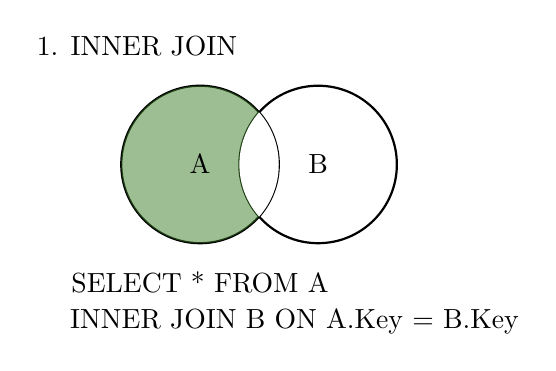
\begin{tikzpicture}
            \node at (-1.3, 0) {1. INNER JOIN};
            \node at (-.5, -3) {\bt{SELECT} * \bt{FROM} A};
            \node at (.7, -3.5) {\bt{INNER JOIN} B \bt{ON} A.Key = B.Key};

            \begin{scope}[shift={(0, -3)}]
                \draw[thick] (-.5,1.5) circle (1);
                \draw[thick] (1,1.5) circle (1);
                \fill[OliveGreen, opacity=0.5] (-.5,1.5) circle (1);
                \node at (-.5, 1.5) {A};
                \node at (1, 1.5) {B};
                \clip (1,1.5) circle (1);
                \fill[white] (-.5,1.5) circle (1);
            \end{scope}
        \end{tikzpicture}
    \end{minipage}
    \hfill
    \begin{minipage}[b]{0.45\textwidth}
        \centering
        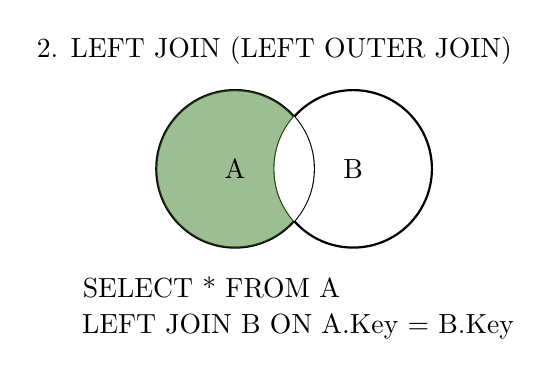
\begin{tikzpicture}
            \node at (0, 0) {2. LEFT JOIN (LEFT OUTER JOIN)};
            \node at (-0.8, -3) {\bt{SELECT} * \bt{FROM} A};
            \node at (0.3, -3.5) {\bt{LEFT JOIN} B \bt{ON} A.Key = B.Key};

            \begin{scope}[shift={(0, -3)}]
                \draw[thick] (-.5,1.5) circle (1);
                \draw[thick] (1,1.5) circle (1);
                \fill[OliveGreen, opacity=0.5] (-.5,1.5) circle (1);
                \node at (-.5, 1.5) {A};
                \node at (1, 1.5) {B};
                \clip (1,1.5) circle (1);
                \fill[white] (-.5,1.5) circle (1);
            \end{scope}
        \end{tikzpicture}
    \end{minipage}
\end{figure}

% RIGHT JOIN
\begin{figure}[htbp]
    \begin{minipage}[b]{0.45\textwidth}
        \centering
        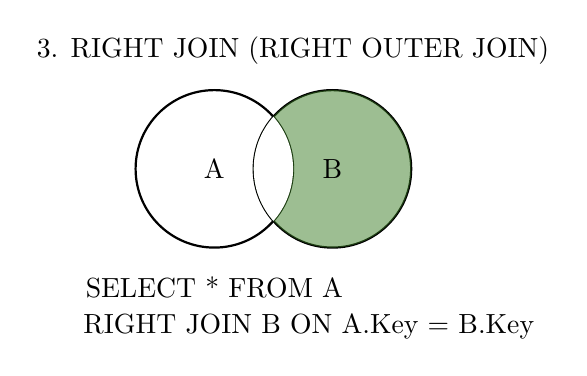
\begin{tikzpicture}
            \node at (.5, 0) {3. RIGHT JOIN (RIGHT OUTER JOIN)};
            \node at (-.5, -3) {\bt{SELECT} * \bt{FROM} A};
            \node at (.7, -3.5) {\bt{RIGHT JOIN} B \bt{ON} A.Key = B.Key};

            \begin{scope}[shift={(0, -3)}]
                \draw[thick] (-.5,1.5) circle (1);
                \draw[thick] (1,1.5) circle (1);
                \fill[OliveGreen, opacity=0.5] (1,1.5) circle (1);
                \node at (-.5, 1.5) {A};
                \node at (1, 1.5) {B};
                \clip (-.5,1.5) circle (1);
                \fill[white] (1,1.5) circle (1);
            \end{scope}
        \end{tikzpicture}
    \end{minipage}
    \hfill
    \begin{minipage}[b]{0.45\textwidth}
        \centering
        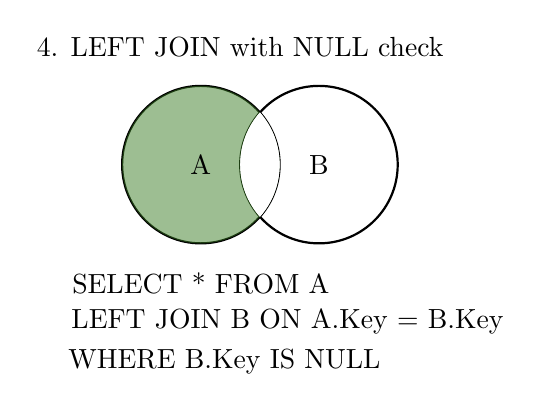
\begin{tikzpicture}
            \node at (0, 0) {4. LEFT JOIN with NULL check};
            \node at (-.5, -3) {\bt{SELECT} * \bt{FROM} A};
            \node at (.6, -3.5) {\bt{LEFT JOIN} B \bt{ON} A.Key = B.Key};
            \node at (-.2, -4) {\bt{WHERE} B.Key \bt{IS NULL}};

            \begin{scope}[shift={(0, -3)}]
                \draw[thick] (-.5,1.5) circle (1);
                \draw[thick] (1,1.5) circle (1);
                \fill[OliveGreen, opacity=0.5] (-.5,1.5) circle (1);
                \node at (-.5, 1.5) {A};
                \node at (1, 1.5) {B};
                \clip (1,1.5) circle (1);
                \fill[white] (-.5,1.5) circle (1);
                \clip (-.5,1.5) circle (1);
                \fill[white] (1,1.5) circle (1);
            \end{scope}
        \end{tikzpicture}
    \end{minipage}
\end{figure}

% RIGHT JOIN with NULL check
\begin{figure}[htbp]
    \begin{minipage}[b]{0.45\textwidth}
        \centering
        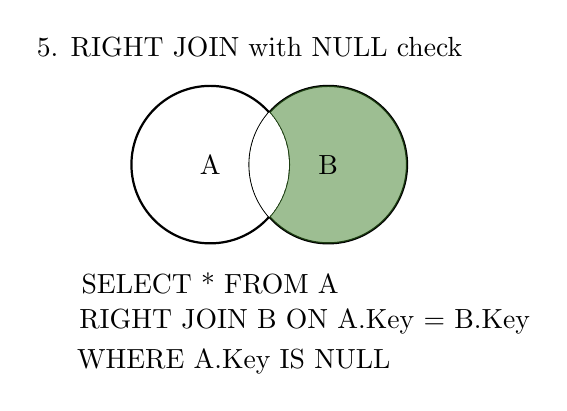
\begin{tikzpicture}
            \node at (0, 0) {5. RIGHT JOIN with NULL check};
            \node at (-.5, -3) {\bt{SELECT} * \bt{FROM} A};
            \node at (.7, -3.5) {\bt{RIGHT JOIN} B \bt{ON} A.Key = B.Key};
            \node at (-.2, -4) {\bt{WHERE} A.Key \bt{IS NULL}};

            \begin{scope}[shift={(0, -3)}]
                \draw[thick] (-.5,1.5) circle (1);
                \draw[thick] (1,1.5) circle (1);
                \fill[OliveGreen, opacity=0.5] (1,1.5) circle (1);
                \node at (-.5, 1.5) {A};
                \node at (1, 1.5) {B};
                \clip (-.5,1.5) circle (1);
                \fill[white] (1,1.5) circle (1);
                \clip (1,1.5) circle (1);
                \fill[white] (-.5,1.5) circle (1);
            \end{scope}
        \end{tikzpicture}
    \end{minipage}
    \hfill
    \begin{minipage}[b]{0.45\textwidth}
        \centering
        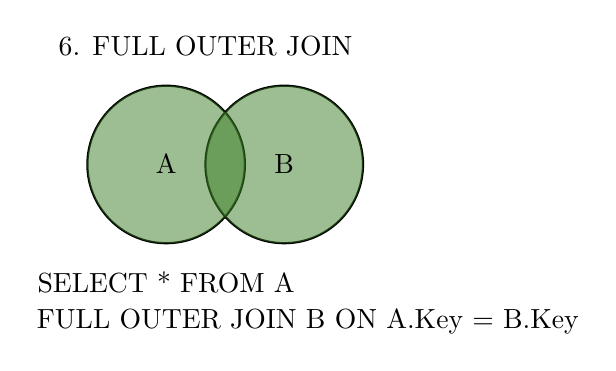
\begin{tikzpicture}
            \node at (0, 0) {6. FULL OUTER JOIN};
            \node at (-.5, -3) {\bt{SELECT} * \bt{FROM} A};
            \node at (1.3, -3.5) {\bt{FULL OUTER JOIN} B \bt{ON} A.Key = B.Key};

            \begin{scope}[shift={(0, -3)}]
                \draw[thick] (-.5,1.5) circle (1);
                \draw[thick] (1,1.5) circle (1);
                \fill[OliveGreen, opacity=0.5] (-.5,1.5) circle (1);
                \fill[OliveGreen, opacity=0.5] (1,1.5) circle (1);
                \node at (-.5, 1.5) {A};
                \node at (1, 1.5) {B};
            \end{scope}
        \end{tikzpicture}
    \end{minipage}
\end{figure}
\begin{figure}[hbt!]
    \centering
    \begin{minipage}[b]{0.45\textwidth}
        \begin{adjustwidth}{.8em}{0pt}
            \noindent
            7. CROSS JOIN\\

            \noindent
            \bt{SELECT} * \bt{FROM} A \bt{CROSS JOIN} B $\equiv$\\
            \bt{SELECT} * \bt{FROM} A \bt{JOIN} B \hspace{3.3em} $\equiv$\\
            $A\times B$ The \textbf{Cartesian product}.\\
        \end{adjustwidth}
    \end{minipage}
    \hfill
    \begin{minipage}[b]{0.45\textwidth}
        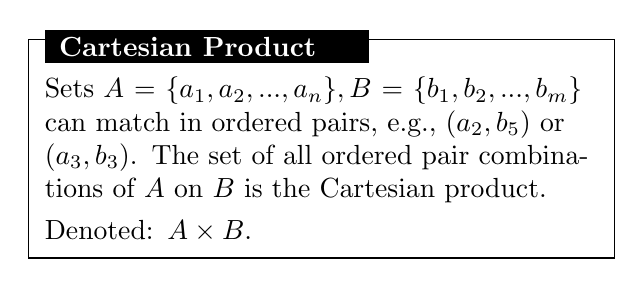
\begin{tikzpicture}
            \node[draw, rectangle, text width=20em, inner sep=6pt, align=left] {
                \vspace{.3em}

                Sets $A = \{a_1, a_2, ..., a_n\}, B = \{b_1, b_2, ..., b_m\}$ can match in ordered pairs, e.g., $(a_2, b_5)$ or $(a_3, b_3)$. The set of all ordered pair combinations of $A$ on $B$ is the Cartesian product. \\
                \vspace{0.3em}
                Denoted: $A \times B$.
            };
            \draw[black, fill=black] (-3.5, 1.1) rectangle (.6, 1.5);
            \node at (-1.7, 1.3) {\textcolor{white}{\textbf{Cartesian Product}}};
        \end{tikzpicture}
    \end{minipage}
\end{figure}

